\chapter*{Conclusions}
\chaptermark{}

Figure~\ref{fig:phisDGsNew} shows the current status of $\phis$ and $\DGs$ measurements. It is an update of Figure~\ref{fig:phisDGs} in
Section~\ref{subsec:intro_Jpsiphi_decay}, which gives an overview of the status in the Spring of 2014, when only results with the 2011
dataset from LHCb were available. Results of the measurement presented in this thesis, which uses both the 2011 and 2012 LHCb datasets and
was published in \cite{LHCb-PAPER-2014-059}, are shown in combination with the results from measurements in the
\BstoJpsipipi~\cite{LHCb-PAPER-2014-019} and \BstoDspDsm~\cite{LHCb-PAPER-2014-051} decay channels. The other results in the figure are
from a new CMS measurement~\cite{CMS:2014jxa}, the updated \atlas{} measurement~\cite{Aad:2014cqa}, and the CDF~\cite{Aaltonen:2012ie} and
D0~\cite{Abazov:2011ry} measurements in the \BstoJpsiphi{} channel.
\begin{figure}[htb]
  \centering
  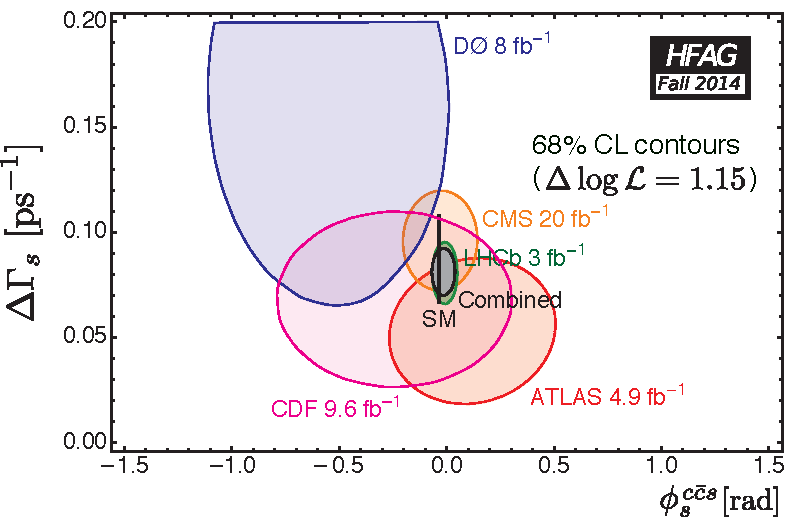
\includegraphics[width=\textwidth]{graphics/results/hfag_Fall2014_DGsphis-cmyk}
  \caption{Combination of $\phis$ (here represented as $\phisccs$) and $\DGs$ measurements by HFAG~\cite{Amhis:2012bh}.
           The estimates at 68\% confidence level (CL) by the different experiments are shown by the coloured contours.
           Note that the LHCb contour (green) is a combination of measurements in the
           \BstoJpsiphi{}, \BstoJpsipipi{}, and \BstoDspDsm{} decays.
           The combined 68\% confidence region is shown by the grey area and the Standard Model prediction by the vertical bar.}
  \label{fig:phisDGsNew}
\end{figure}

The objective of these measurements, as described in Sections~\ref{sec:intro_SM}--\ref{sec:intro_Jpsiphi}, is to test the Standard Model by
comparing the CP violation that is measured in $\btoccs$ transitions to the prediction obtained by interpreting other measurements within
the Standard Model framework. The current combined precision of the $\phis$ result is 0.04\unitsp{}rad, which is equal to the deviation of
the Standard Model prediction from zero. This precision is not yet sufficient to measure potential small deviations from the Standard
Model, but these measurements do rule out large contributions from non-Standard Model physics. As discussed in
Section~\ref{subsec:intro_Jpsiphi_decay}, both experimental and theoretical improvements are required for a more precise analysis of CP
violation in $\btoccs$ transitions.

At lowest order, the decays that are included in the combination of Figure~\ref{fig:phisDGsNew} are governed by a single tree-level
$\btoccs$ transition and CP violation is described by common $\phis$ and $\lamsAbs$ parameters. To compare a more precise measurement of CP
violation to its prediction in the Standard Model, higher order (penguin) contributions must be considered. These potentially yield CP
violation parameters with different values for each decay and each angular-momentum state contributing to the \BstoJpsiKK{} decay.

A close interplay between theory and experiment will be required to interpret a precise measurement of these CP-violation parameters.
Calculations of their values (see e.g. \cite{Liu:2013nea}) suffer from uncertainties in the strong interactions within the involved
hadrons. However, by exploiting approximate symmetries between different decays of $\Bd$ and $\Bs$ mesons, a framework of measurements
and calculations can be built to interpret the experimental results~\cite{Faller:2008gt,DeBruyn:2014oga}. Both precise measurements and
precise estimates of how the symmetries between different decays are broken are required for such an analysis.

In reference~\cite{DeBruyn:2014oga} it is proposed to use the interplay between the decays \BstoJpsiphi, \BstoJpsiKS, \BstoJpsiKst,
\BdtoJpsiKS, and \BdtoJpsirho{} for an analysis of CP violation in $\btoccs$ and $\btoccd$ transitions. For both the \BstoJpsiphi{} and
\BdtoJpsirho{} decays measurements of CP violation per intermediate angular-momentum state is required in this framework. The results of
the first measurement in this format for the \BstoJpsiphi{} channel was presented in Chapter~\ref{chap:result} (see also
reference~\cite{LHCb-PAPER-2014-059}).

While the current CP-violation results are still compatible with both the Standard Model and no CP violation, it is expected that the
measurement with future LHCb data will start to distinguish between the Standard Model and other scenarios. With the final dataset of the
LHCb experiment an increase in precision of roughly an order of magnitude is expected~\cite{CERN-LHCC-2011-001,LHCB-PAPER-2012-031}. This
improvement has to come from an increased number of decays produced by the LHC, but also from improvements in the analysis procedure.

For the \BstoJpsiphi{} decay, the statistical precision of the CP-violation measurement can be improved by a decreasing the probability for
an incorrect flavour tag. Given a wrong-tag probability of 40\%, a 10\% improvement of this value gives almost a factor two increase in the
effective number of perfectly tagged decays (see also Section~\ref{subsec:ana_tagging_impl}). Potential improvements of the flavour-tagging
procedure include the use of more sophisticated (multivariate) techniques to select and analyse tagging particles, the development of
additional tagging algorithms, and an improved understanding of the properties of particles that are created in association with $\Bs$
mesons.

With improved statistical precision, also the systematic uncertainties in the measurement must be reduced to gain in overall precision. 
